% Title: Report LaTex File: Concept Development
% Auther: DC Eksteen
% Student Number: 22623906
% Contact: 22623906@sun.ac.za
% Date: 2022/09/22
% Version: 2.0

\chapter{Concept Design and Evaluation}
% Section overview:

\color{red}

This section aims to identify and refine any requirements that were required of the training platform, and then demonstrate and analyse a concept solution that will be expanded into the final delivered demonstration model in further sections. Table \ref{tab:conditions} shows the user requirements that were derived from the project objectives and literature review. These user requirements are then analysed in Section \ref{sec:req} to get engineering requirements and technical- and functional performance measures.

\begin{table}[H]
	\centering
	\caption{Derived User Requirements}
	\begin{tabularx}{\textwidth}{>{\raggedright}p{1 cm} X >{\raggedright\arraybackslash}p{2cm}}
		\toprule
		\multicolumn{2}{c}{User Requirement} & Priority                            \\
		\midrule
		UR 1                                 & Connect with Zwift      & Essential \\
		UR 2                                 & Controllable Resistance & High      \\
		UR 3                                 & Cadence Measurement     & Medium    \\
		UR 4                                 & Power Measurement       & Low       \\
		\bottomrule
	\end{tabularx}
	\label{tab:conditions}
\end{table}

\color{black}

\newpage

\section{Expected Operating Conditions}
\subsection{Operating Speeds}
\label{sec:opspeedc}

The typical speed of a cyclist typically ranges from \SI{10}{\kilo\meter\per\hour} to \SI{50}{\kilo\meter\per\hour} when cycling on reasonably flat ground. For the design of the platform, a speed of maximum required speed of \SI{60}{\kilo\meter\per\hour} was assumed.

Typically, amateur cyclists maintain an average power output between \SI{75}{\watt} and \SI{100}{\watt}, and pro cyclists can maintain up to \SI{400}{\watt}, during a 1 hour workout. As the cyclist's speed increases, less torque is required to maintain the same power output. The relation is expressed as Equation \ref{eq:pow}.

\subsection{Torque Requirements}

The required braking torque range is dependant on the cycling speed and the power output of the cyclist.

When considering the \SI{90}{\milli\meter} roller size that was selected in Section \ref{sec:opspeedc}, the Torque requirements for different power outputs is shown in Figure \ref{fig:torqueCalcc} below. From the figure, it can be seen that the torque requirement at low speeds will dominate the torque requirement and should thus be used as consideration when selecting torque requirements of the brake.

\newpage

\section{Requirement Analysis}
\label{sec:req}

\begin{itemize}
	\item Zwift controllable smart trainer
	\item Inexpensive
	\item Easily accessible by many consumers
	\item Comparable features to existing models.
\end{itemize}

\section{Concept Design}
\label{sec:conc}


\begin{figure}[H]
	\begin{center}
		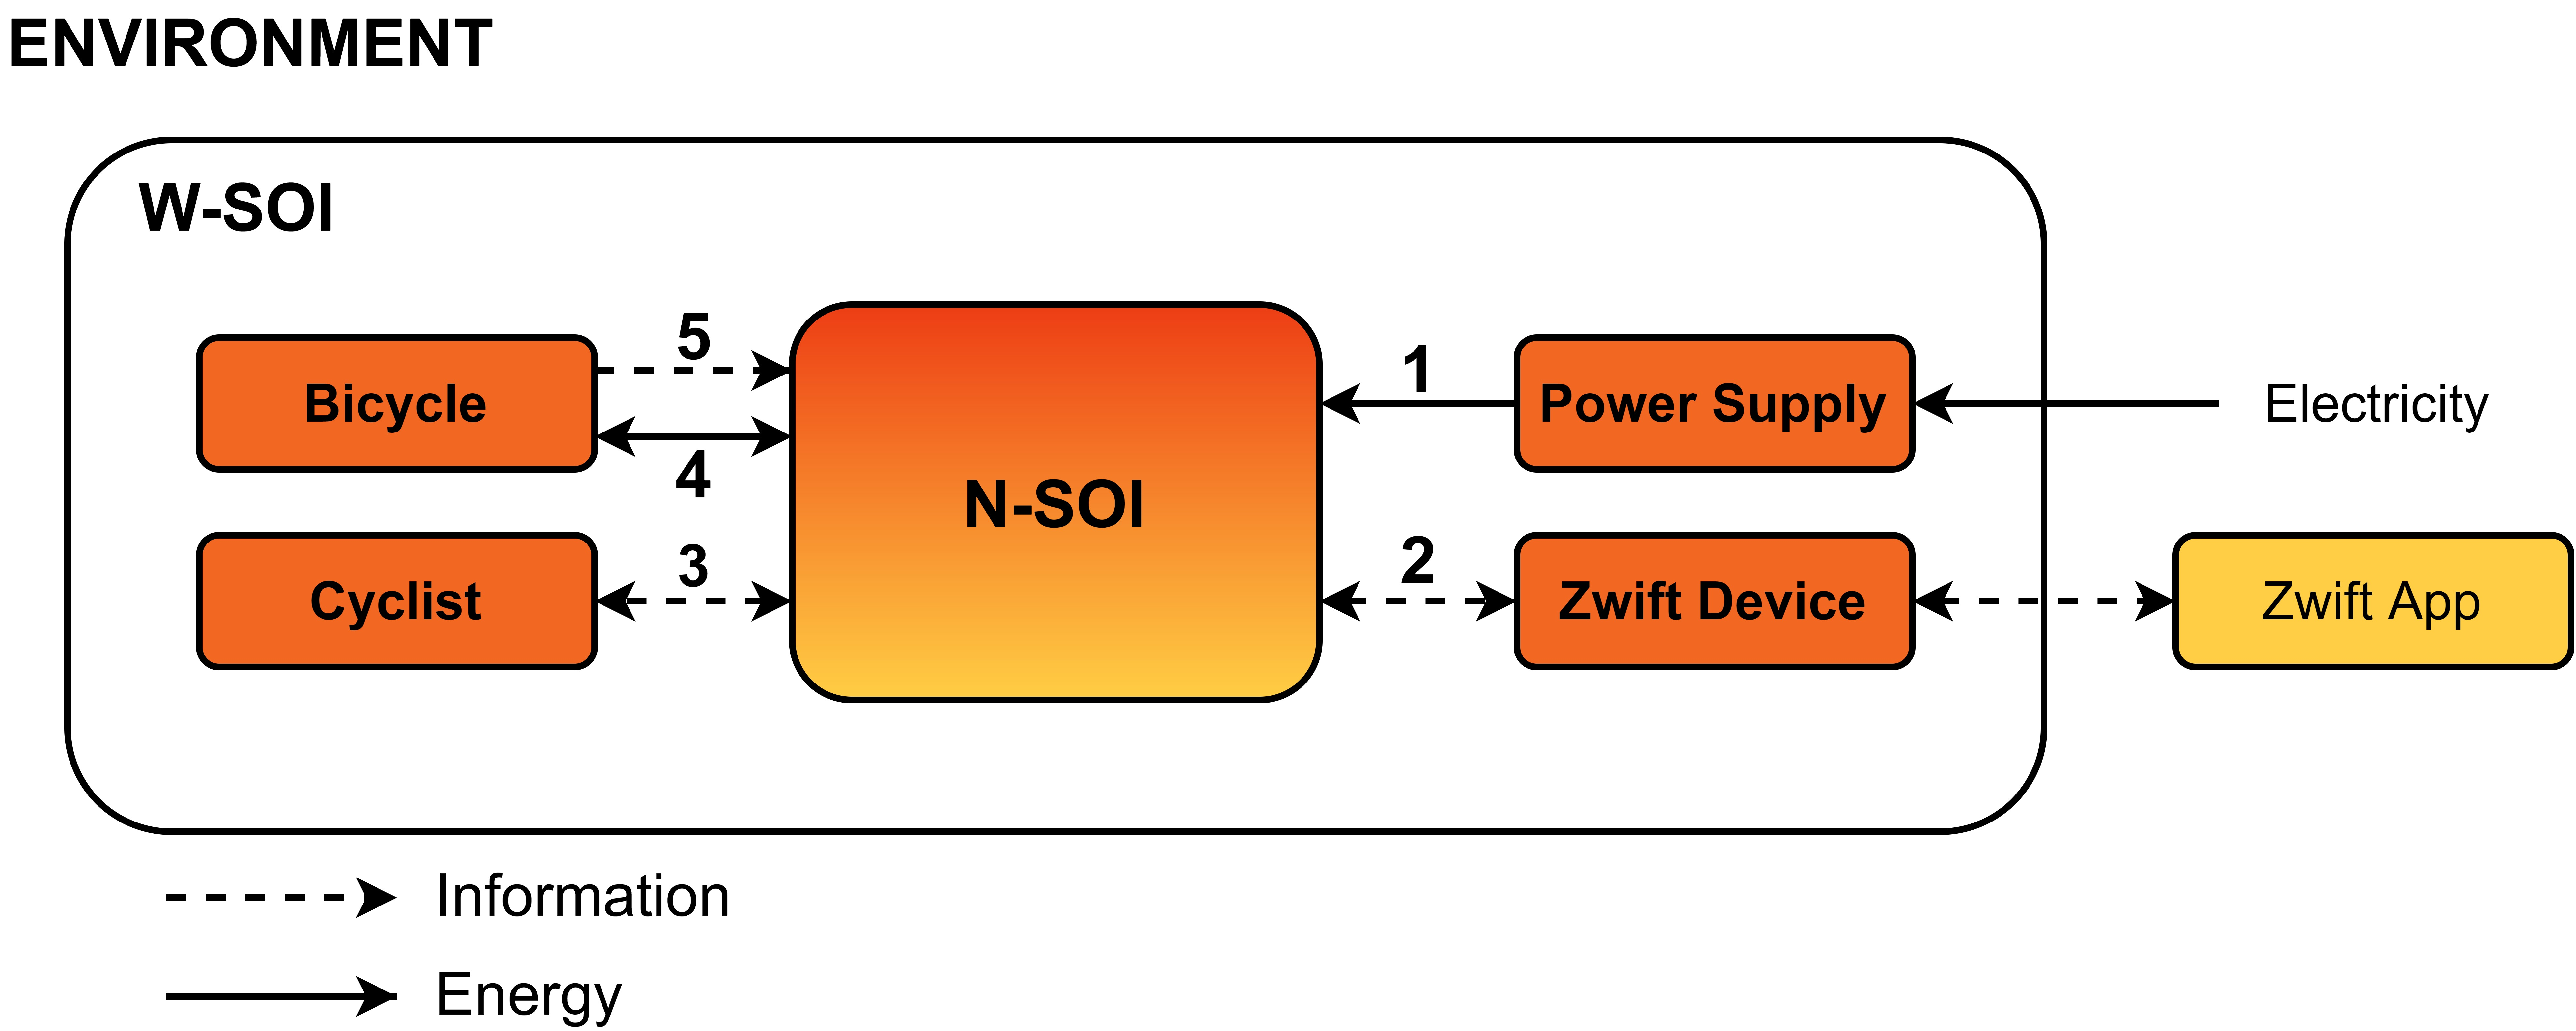
\includegraphics[width=0.8\textwidth]{SOI.jpg}
		\caption{Concept Boundary of Interest}
		\label{fig:soi}
	\end{center}
\end{figure}


\section{Concept Evaluation}
\label{sec:eval}